\newpage
\chapter{Approach}
\label{sec:approach}
The role mining problems (see section \ref{sec:roleMiningProblems}) have been approached with different problem formulations, techniques and algorithms. In this thesis the approach of solving role mining with an evolutionary computation approach is investigated. \hl{An evolutionary computation has the advantage of ... , which is needed for RoleMining.}

Since there has not been a lot of research done up till now regarding Role Mining with evolutionary computation (see chapter \ref{sec:relatedWork} for related work), the research in this thesis starts with a basic set up of the domain-specific problem as evolutionary computation problem. The evolutionary algorithms, the representation of an individual, variation operators, selection mechanisms and fitness functions used in this approach are described in the following sections. \hl{For handling constraints for an RBAC$_2$ role model, a penalty function and intelligent variation operators are introduced. In order to come to an human digestible representation of individuals for human feedback in an IEC approach, an alternative approach with a different representation and a Co-Evolution technique is presented.}

	\section{Evo-RoleMiner and Evo-RoleMiner$M$}
	In this thesis a single- and a multi-objective EA for Role Mining has been constructed, where the objectives can be exchanged in regard to the considered Role Mining Problem. In the following the algorithms will be called Evo-RoleMiner and Evo-RoleMiner$M$ accordingly.
	
	The Evo-RoleMiner is based on the evolutionary algorithm process described in chapter \ref{sec:EA}. A pseudo-code is outlined in Algorithm \ref{alg:EA} in the Appendix.
	
	The Evo-RoleMiner$M$ is based on the NSGA-II algorithm described in section \ref{sec:nsga2}. The second version of the Evo-RoleMiner$M$ is based on the improved NSGA-II$R$ algorithm from Fortin et al.\cite{Fortin:2013} (see also section \ref{sec:crowdingDistance}). In a third version of the Evo-RoleMiner$M$ the second of two objectives can be relaxed by setting a weight (see also section \ref{sec:weightedNSGA2}). The third version builds on version two of the Evo-RoleMiner$M$ and is based on NSGA-II$R$ with weights.
    
    \section{Representation of a Role Model as Individual}
    The representation of individuals in an EA is crucial for the success of the EA and influences the variation operators. Finding a good representation of role models as individuals for a Role Mining EA is a challenging task, since the number of roles for a role model is not necessarily predefined and part of the search. After considering a bit-string representation and the multi-chromosomal representation proposed by Saenko \& Kotenko\cite{Igor} (see Appendix \ref{sec:A_representations}), the improved representation proposed by Saenko \& Kotenko\cite{saenko2012design} has been chosen as representation of individuals. One of the drawbacks of the other representations are unnecessary information (unused roles). Another disadvantage of the representations are complex crossover operations.
    
    The improved representation eliminates these drawbacks by having one chromosome for an individual, where no unnecessary information occur. The chromosome consists of a list of roles, which contain a user-list and a permission-list (see figure \ref{fig:representation3}). For the Evo-RoleMiner and Evo-RoleMiner$M$ the user- and permission lists are implemented as sets.
        
    \begin{figure}[H]
        \centering
        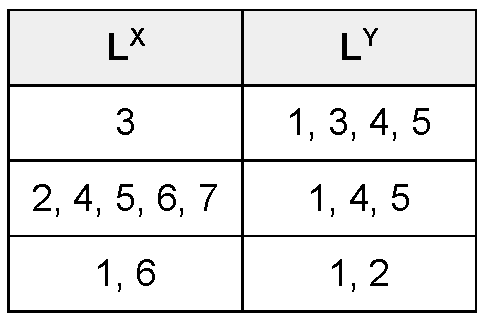
\includegraphics[scale=0.4]{ComplexRepresentation2}
        \caption{Example of a role model representation suggested in Saenko \& Kotenko\cite{saenko2012design}. A row represents a role (gene). In the column $L^X$ are user lists and in the column $L^Y$ are permission lists.}
        \label{fig:representation3}
    \end{figure}
    
    \section{Variation Operators on Role Model Representation}
    Dependent on the choice of the representation of individuals in the previous section, according mutation and crossover methods are created. The choice of variation operators and how often they are executed influences how much of the search space is discovered during the evolution. Since the improved representation of Saenko \& Kotenko\cite{saenko2012design} has been selected for this thesis, the following variation operators are suited for this representation.
    
        \subsection{Mutation methods}
        Since no further instructions for the mutation are given in Saenko \& Kotenko\cite{saenko2012design}, the mutation operations have been chosen intuitively. For the mutation six different mutation types are implemented:
        
        \begin{itemize}
            \setlength{\itemsep}{1pt}
            \item Add a new role
            \item Add a user to a role
            \item Add a permission to a role
            \item Remove a role
            \item Remove a user from a role
            \item Remove a permission from a role
        \end{itemize}
        
        Examples can be seen in Figure \ref{fig:mutationOperations}. Which role, user or permission is added or removed is chosen randomly. If an individual gets mutated is determined by a fixed probability $MUTPB$. In addition, fixed probabilities for each mutation method are dictating how the individual gets mutated. The probabilities allow to influence how often a certain mutation should be executed and can therefore influence how much new solutions are discovered and how likely good solutions are lost. Furthermore the probabilities of adding or removing a role could be set to 0 for the Min-Noise-RMP (see section \ref{sec:roleMiningProblems}).
        
        \begin{figure}[H]
              	\centering
              	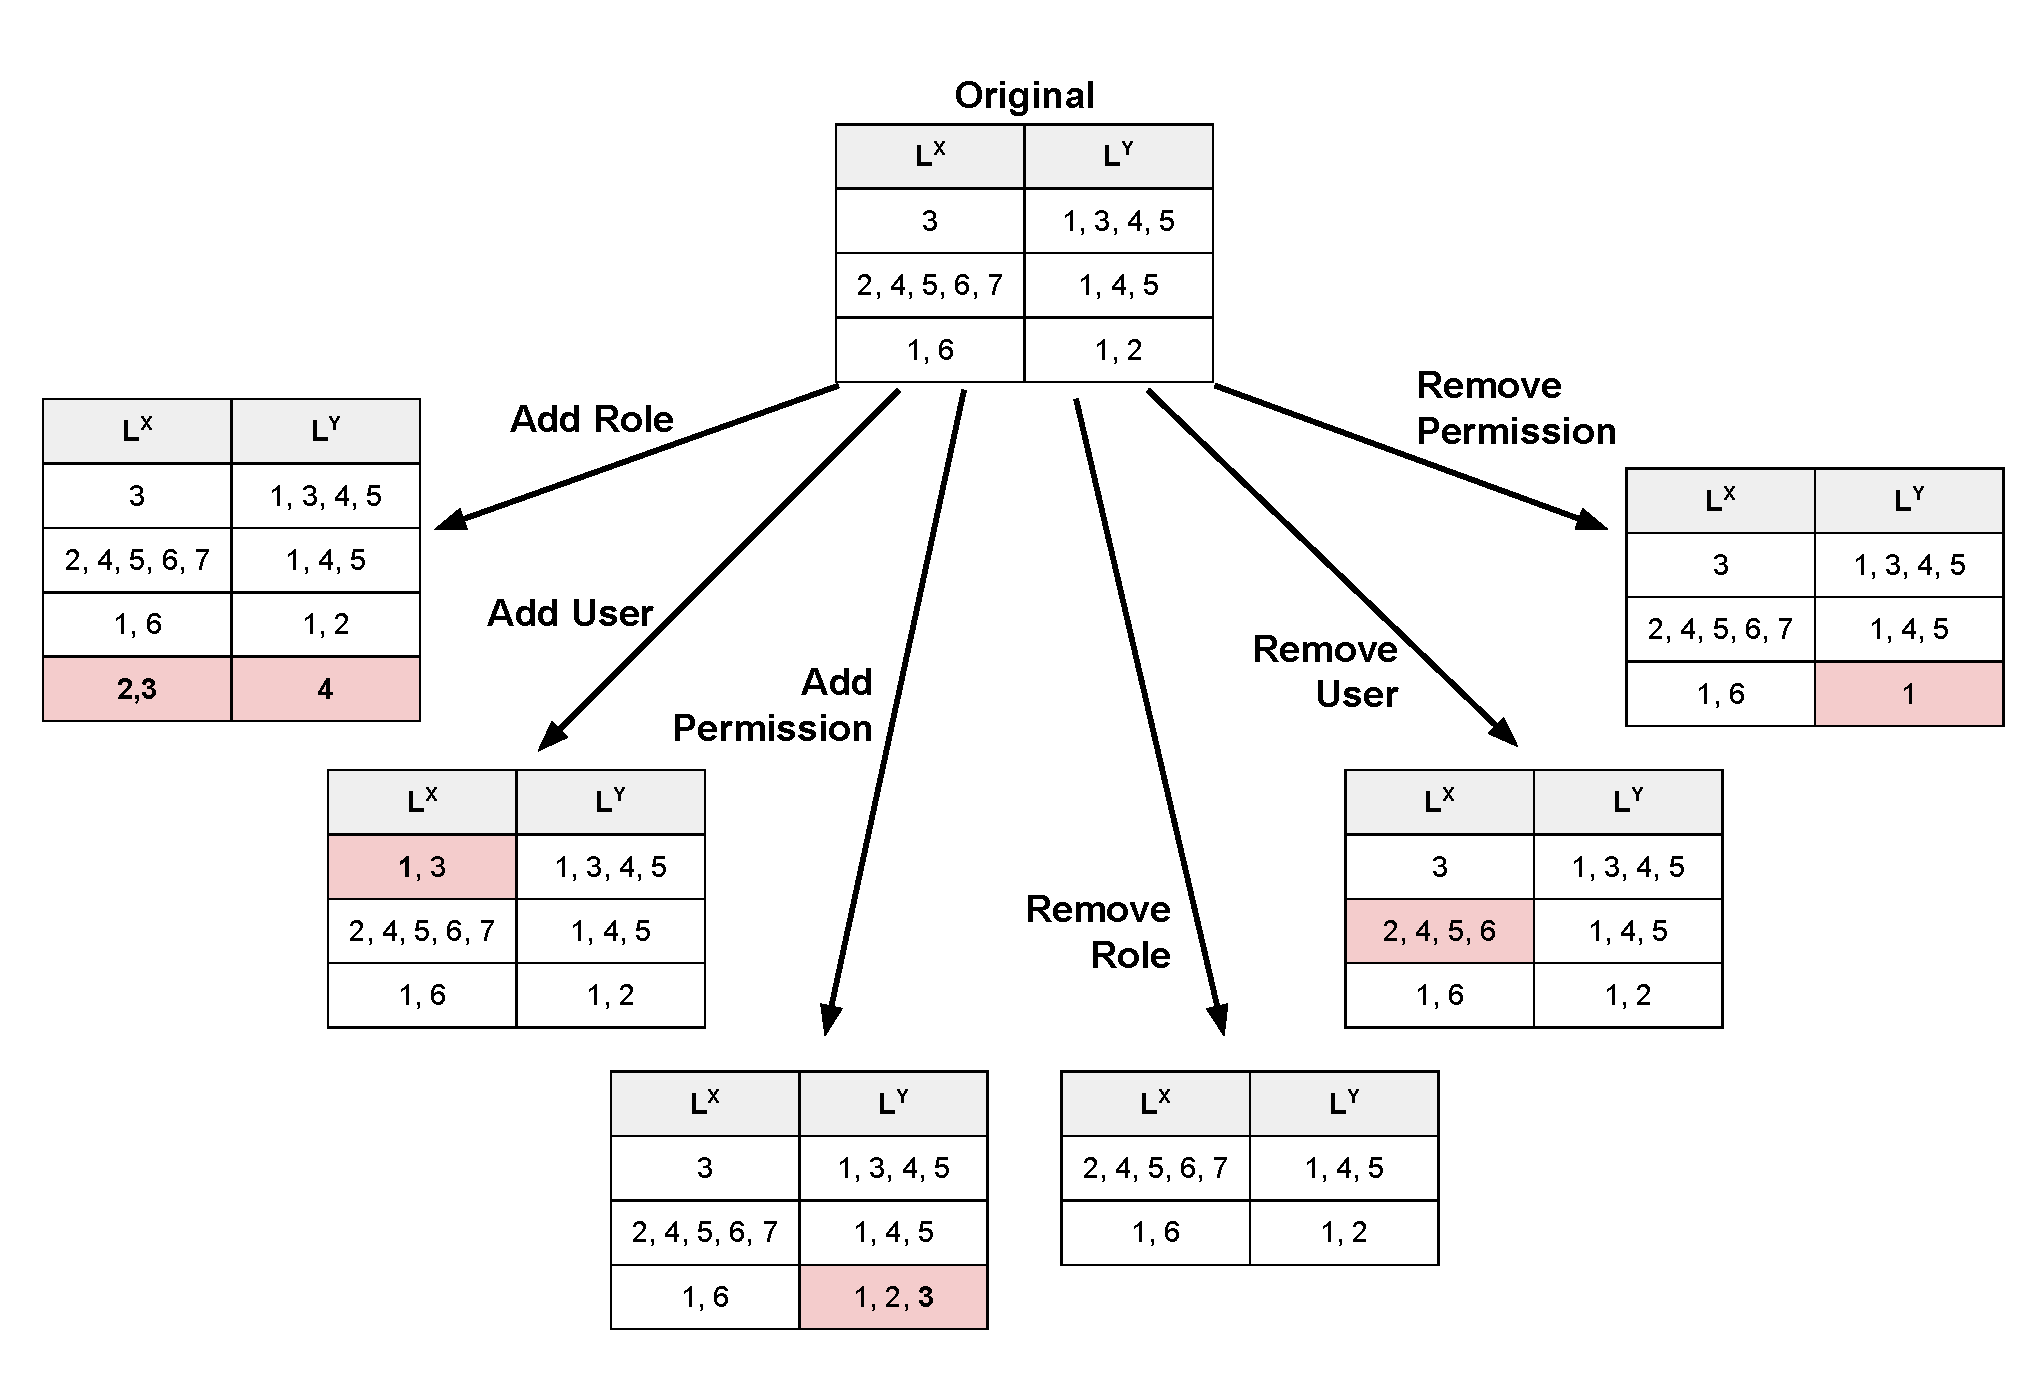
\includegraphics[scale=0.27]{Mutations}
              	\caption{Examples for the six different mutation operators}
              	\label{fig:mutationOperations}
        \end{figure}
                
        There are two implementation variations of the mutation operations. In the first implementation, mutation towards an incomplete role model is allowed. An incomplete role model is a role model where users with no role assignments and permissions not contained in any role can occur.
       
        The second implementation prevents that incomplete role models with missing users or permissions can occur. This is ensured by re-executing the mutation type. For example if the mutation of removing a user would lead to a role model where the user has no role assigned, the mutation is discarded and executed again, where a different user is randomly chosen. If all users only have one role assigned, the reverse mutation (in this case adding a user) is executed. To prevent deadlocks, this reverse-switch is only allowed once. This second implementation of mutation operations restricts the search space. 
        
        \subsection{Crossover methods}
        The recombination used for the Evo-RoleMiner and Evo-RoleMiner$M$ is like in Saenko \& Kotenko\cite{saenko2012design} executed on two individuals with a traditional one-point crossover: Both individuals are keeping their first $x$ roles, while the rest of the roles get exchanged as shown in figure \ref{fig:crossover}. The points of crossover (after $x$ roles) of the two individuals are randomly chosen.
        
        \begin{figure}[H]
            \centering
            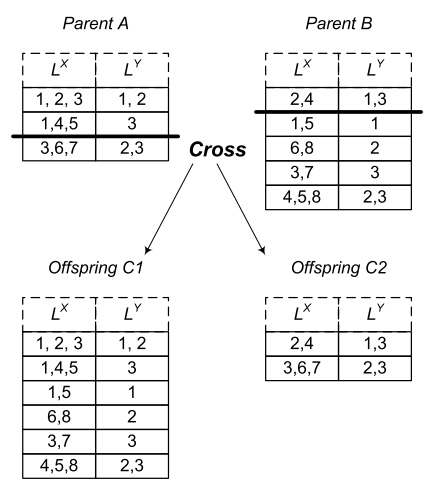
\includegraphics[scale=0.8]{crossover.png}
            \caption{Examples of the crossover in the improved GA for the RMP by Saenko \& Kotenko\cite{saenko2012design}}
            \label{fig:crossover}
        \end{figure}
        
        As for mutation there is also a fixed probability $CXPB$ for crossover operations. It should be noted that the crossover operation can lead to incomplete role models, where users might not get any role assigned or permissions are not contained in any role. While the prevention of incomplete role models is straight forward in the mutation operations, this assurance is less straight forward in the crossover operation.
        
        \subsection{Local optimization}
        \label{sec:localOptimization}
        A mutation and crossover is always followed by a local optimization on the individual. Like in Saenko \& Kotenko\cite{saenko2012design} the individual is compressed by the rule of User combining and/or Permission combining. If there are roles with the same user sets, they get combined by merging the permissions sets (User combing). Accordingly roles get combined by merging user sets when the same permission sets are present (Permission combining). It should be noted that by this compression the number of roles in the role model can shrink. Furthermore the order of first user combining and then permission combining might not necessarily optimize the individual the best possible way (see example in Figure \ref{fig:localOptimization}b).
        
        \begin{figure}[H]
            \centering
            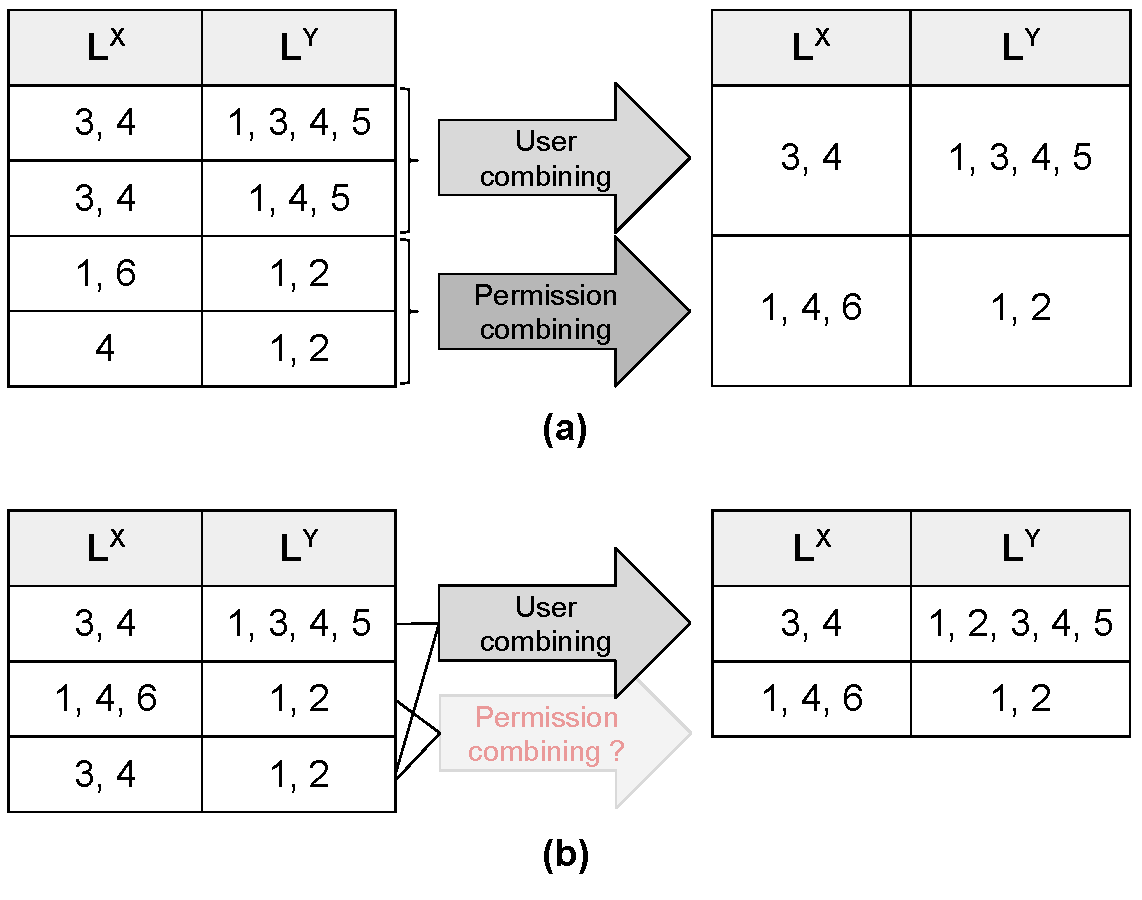
\includegraphics[scale=0.3]{LocalOptimization}
            \caption{Examples of local optimizations. In (a) a case for user- and a separate case for permission-combining is detected and executed. In (b) an overlapping user- and permission-combining is detected, but only the user-combining is executed.}
            \label{fig:localOptimization}
        \end{figure}
        
        In the Evo-RoleMiner and Evo-RoleMiner$M$ this local optimization can be switched on and off by the parameter "optimization".
        
    \section{Selection Strategy}
    Which selection mechanisms are chosen is dependent on if a single-objective or a multi-objective EA is applied. 
    For the parent selection in the Evo-RoleMiner a tournament selection is chosen since it is a widely used selection strategy in EA (see section \ref{sec:parentSelection}). With the tournament size $k$ the selection pressure can be adjusted. The same selection strategy is chosen for the survivor selection in the Evo-RoleMiner.
    
    For the Evo-RoleMiner$M$ the selection strategy is dictated by the NSGA-II and NSGA-II$R$ (see section \ref{sec:nsga2} and \ref{sec:crowdingDistance}), where the parent selection is based on a binary tournament selection and the survivor selection is executed on the population of the parent population $P_P$ and the offspring population $P_O$.
    
    \section{Measuring the Interpretability of Roles}
    \label{sec:meaningfulness}
    The goal is to generate a role model, which is accepted by the business, in particular the security administrators. Therefore an appropriate measure has to be found. The interpretability of a role shall express how easy a reasonable interpretation of the role can be identified, such that the role gets adopted by security administrators. An interpretable role is also called a "meaningful" role.
    
    The interpretability of a role in this thesis is measured with the help of user attributes. One or more user attributes can describe the users of a role. For example:
    
    \storestyleof{itemize}
    \begin{listliketab}
        \begin{tabular}{ll}
            Let     &  $OrganizationalUnit \in \{HumanResources, Sales, Motor\}$,\\
                    &  $Location \in \{Denmark, Germany, US\}$ and\\
                    &  $EmployeeType \in \{Internal, External\}$\\
                    &  be the user attributes.  
        \end{tabular}
    \end{listliketab}
    
    The users of a role can be described by an AND-combination of the attribute values, e.g. $Sales \wedge Denmark$ when all users in the role are in $Sales$ and $Denmark$. For simplicity an OR-combination, e.g. $Sales \vee Motor$ where all users would be either in $Sales$ or $Motor$, is not considered. This case can be rather represented by two roles with the same permission-set, but different user-sets. It should be noted that this requires the disabling of the permission-combining optimization (see section \ref{sec:localOptimization}).
    
    \iffalse
    A similar approach is followed in Xu \& Stoller\cite{Xu}, but they calculate an attribute mismatch of roles, which does not consider the heterogeneity of users in different roles as well as homogeneity of users in the same role. In the following sections two approaches are discussed theoretically and one of the approaches is implemented.
    
    \fi
    Two approaches have been considered to measure how well a role can be described by the user attribute values of its user-members. In the following both approaches are introduced, where the later one got implemented.
    
        \subsection{Role Cluster Approach}
        One approach is to treat roles like clusters where the users and their attribute values are objects. A role-cluster is considered good if the user-objects within the role-cluster are compact and the user-objects between role-clusters are separated. This means that the user attribute values considered describe all users within a role (compactness), but no users not in the role (separation). The compactness and separation of a role-cluster can be measured with the average silhouette coefficients of the user-objects of a role-cluster\cite{Han}. If the silhouette coefficient of an user-object approaches 1, the role-cluster, the user is assigned to, is considered compact and the user-object is far away from other role-clusters. A negative silhouette coefficient says that the user-object is closer to user-objects of other role-clusters than to user-objects of the same role-clusters.
        
        This measure of the average silhouette coefficients requires the role-clusters to be crisp, which means a user-object can be only in one role-cluster. But since the users can have several roles the role-clusters are fuzzy. Furthermore the measure has to be executed for every user attribute combination. Therefore an altered calculation of silhouette coefficients has to be used or a different measure has to be used to evaluate the role-clusters. To evaluate fuzzy clusters the sum of the squared error (SSE) can be used\cite{Han}. It measures how well a fuzzy clustering fits a data set. In Rawashdeh \& Ralescu\cite{rawashdeh2012fuzzy} the authors suggest an algorithm for the silhouette coefficient in fuzzy clusters.
        
        The role-cluster approach has not been followed further.
        
        \subsection{Role Classifier-Rule Approach}
        \label{sec:classifierRule}
        Another approach is to generate classifier-rules for roles and measure the accuracy of these rules. Additionally the rule should be simple and not too complex (e.g. many conditions, which identify exactly one user). For this supervised-learning approach, all users in a role get classified as being in the role, while all other users are classified as being not in the role. Hence for each role a binary classification problem has to be solved.
        
        Rules can be extracted from a decision tree or can obtained directly using a Sequential Covering algorithm\cite{Han}. In traditional decision tree construction like ID3 or C4.5 the dataset gets repeatedly splitted based on the attribute which most effectively splits the dataset in one class or the other. The depth of the tree could be used as the measure of a rule.
        
        The split by information gain is not necessarily wanted for the rules describing a role, since permissions originally have not been assigned to users which share the most common user attribute values, but rather because users gained legitimation through other specific attribute values. For example although users in a generated role are all located in $Denmark$, while users not in the role are located elsewhere, the reason that users of the role got assigned to the permission set the generated role is grouping could be due to the Departments they are in, which could be diverging. The information gain for the location would be higher, but not necessary the legitimation, why a user gets the permission set assigned through the role. Also the measure used for splitting the data in a decision tree is often biased towards class imbalances or multivalued attributes\cite{Han}.
        
        Furthermore classifier-rules for both classes are discovered, while for the measuring of the role only the rules for class "\textit{In the role}" are from interest. Therefore an application-specific algorithm has been created to discover the most descriptive rules for a role (class "\textit{In the role}").
        
        The algorithm got inspired by Sequential Covering algorithms, which directly learns rules for classification by repeatedly removing a portion of the dataset. In the following the algorithm for rule induction is described. The according pseudo-code of the algorithm can be seen in Algorithm \ref{alg:ruleInduction}.        
        
        \begin{algorithm}
        	\small
            \caption{Rule induction algorithm for classifier-rules for roles\protect\\
            $D$ = List of role members, which are not matched by current rule\protect\\
            $RM$ = List of users, which are member of the role\protect\\
            $notRM$ = List of users, which are not members of the role\protect\\
            $rule$ = Current rule\protect\\
            $max$ = Maximum allowed rule size (number of OR-connected rules)\protect\\
            $PB_{notRM}$ = Probability that rule matches a user in $notRM$\protect\\
            $PB_{RM}$ = Probability that rule matches a user in $RM$}
            \label{alg:ruleInduction}
            \begin{algorithmic}[1]
                \Procedure{ruleInduction}{$D$,$RM$,$notRM$,$rule$,$max$}
                    \State $allAttrSets$ = Create all combinations of attributes
                    \State sort($allAttrSets$)
                    \State $ruleSet$ = []
                    \While{ $len(D) > 0$}
                        \State $member = D.pop()$
                        \While{ $len(allAttrSets) > 0$}
                            \State $attrSet = allAttrSets.pop()$
                            \State $newRule$ = \textsc{createRule}($attrSet$,$member$)
                            \State $rule$.add($newRule$)
                            \State $PB_{notRM}$ = \textsc{calculateProbabilityInClass}($rule$,$notRM$)
                            \If{ $PB_{notRM} <= (1/3)$}
                                \State $PB_{RM}$ = \textsc{calculateProbabilityInClass}($rule$,$RM$)
                                \State Remove users in $D$, which are matching $rule$
                                \If{ $PB_{RM} >= (2/3)$}
	                                \State $ruleSet$.append($rule$,$PB_{RM}$,$PB_{notRM}$)
	                                \If{ $PB_{RM} == 1$ AND $PB_{notRM} == 0$}
	                                \State $allAttrSets$ = \textsc{reduceAllAttrSet}($allAttrSets$, $rule$)
	                                \EndIf
                                \Else
                                    \If { $size(rule) <= max$}
                                        \State ... recursion ...
                                        \iffalse
                                        \State $extendedRules$ = ruleInduction($D$,$RM$,$notRM$,$rule$,$max$)
                                        \For {$extendedRule$ in $extendedRules$}
                                            \State $ruleSet$.append($extendedRule$)
                                            \If{ $PB_{RM} == 1$ AND $PB_{notRM} == 0$}
                                                \State $allAttrSets$=\textsc{reduceAllAttrSet}($allAttrSets$, $rule$)
                                            \EndIf
                                        \EndFor
                                        \fi
                                    \EndIf
                                \EndIf
                            \EndIf
                        \EndWhile 
                    \EndWhile
                    \State \Return $ruleSet$
                \EndProcedure
            \end{algorithmic}
        \end{algorithm}
        
    Before the algorithm is applied on a role, all users of the role in the role model get classified as "\textit{In the role}" or "\textit{Not in the role}". A set of all user attribute combinations is created (see line 2 in pseudo-code). If $X$ user attributes are considered, $2^X-1$ combinations are created. For example with the user attributes $Department$ and $Location$, the following combinations are possible:
    
    \centerline{($Department$), ($Location$), ($Department$, $Location$)}
    
    The first user in the role is picked and a the smallest user attribute combination (for example ($Department$)) is chosen (line 6). A rule is generated out of the user attribute values of the user for the chosen user attributes (line 7). In the example the $Department$ the user is in, creates a rule, i.e. $rule$=($HumanResources$).
    
    Next it will be checked if users not in the role also comply with the rule (line 11). If too many users outside the role also comply with the rule, the rule is discarded. Basically the sensitivity of the rule according to class "\textit{Not in the role}" is calculated and checked if it is beneath a specified threshold $t1$ (currently set to $t1$=$\frac{1}{3}$). If the rule persists the check (line 12), it is measured how many users inside the role comply with the rule (line 13). Again the sensitivity is calculated, but this time on the users in class "\textit{In the role}". Also all users inside the role, which comply with the rule, are not considered any further and are removed (line 14). If a certain threshold $t2$ is met (currently set to $t2$=$\frac{2}{3}$) (line 15), the rule is considered as a potential classifier-rule for the role (line 16).
    
    The next user left in the role is picked (line 2) and a the smallest user attribute combination left (for example ($Location$)) is chosen (line 8) and the procedure continues as described above until no user attribute combinations or users are left.
    
    Certain user attribute combinations get removed when the potential rule yields a perfect potential rule, which is when the rule is complying with all users inside the role and with none of the users outside the role (line 17). The user attribute combinations, where the perfect potential rule is a subset of, get removed (line 18). If the potential rule is not perfect, a more complex user combination might yield a better potential rule and is kept as possibility in the user attribute set.
    
    If the threshold $t2$ is not met (percentage of users inside the role comply with the rule is too low), the potential rule gets eventually extended by another OR-connecting rule by calling the procedure recursively (line 21). This can be specified by the parameter $max$ in the algorithm. By setting $max$=2 an OR-connecting rule like $Department=HumanResources \vee Department=Sales$ can be constructed.
    
    After generating the rules for a role, the rule with the best accuracy gives the measure for the role interpretability ("meaningfulness"). The accuracy of a rule is measured by
    
    \begin{equation}
    accuracy = \frac{TP+TN}{P+N}
    \end{equation}
    
    where:
    
    \begin{itemize}
    	\item $TP$ are the true positives, meaning the number of users classified as "\textit{In the role}" by the rule
    	\item $TN$ are the true negatives, meaning the number of users classified as "\textit{Not in the role}" by the rule
    	\item $P$ are the true positives, meaning the number of actual users in the role
    	\item $N$ are the true negatives, meaning the number of actual users not in the role
    \end{itemize}
        
    \section{Objective Measures}
    \label{sec:objectiveMeasure}
    Several objective measures of the role mining problems (see section \ref{sec:roleMiningProblems}) are implemented for the Evo-RoleMiner and the Evo-RoleMiner$M$ in order to measure the individuals of a population. The implemented objective measures introduced in the following are organized in the according role model categories: Completeness, Complexity and Comprehension (see section \ref{sec:rmQuality}).
    
    \subsection{Completeness Measures}
    \label{sec:optimizationCompleteness}
    To measure the completeness (see section \ref{sec:completeness}) different measures can be created. All of them need the original access control policies $UPA$ for measuring how complete the current considered role model is.
    
    \begin{itemize}
    	\item \textbf{Confidentiality Violations}\\
    	Confidentiality violations exist when users get more permissions in the generated role model, than they had in the original access control policies (overentitlements). These violations are measured by counting the additional set positive bits ("1") in the resulting matrix of $UA \times PA$ with $UPA$. 
    	For minimizing confidentiality violations the worst case would be the count of all negative bits in $UPA$, meaning that everyone gets all permissions. The best case is to have zero confidentiality violations.
    	
    	\item \textbf{Availability Violations}\\
    	In contrast to confidentiality violations, availability violations exist when users get less permissions in the generated role model, than they had in the original access control policies (underentitlements). Also here the measure is executed by comparing the resulting matrix of $UA \times PA$ with $UPA$, but in this case the negative bits ("0") are counted.
    	For minimizing availability violations the worst case would be the count of all positive bits in $UPA$, meaning that no one gets the permissions they had in the original access control policies. The best case is to have zero availability violations.
    	
    	\iffalse \item \textbf{Confidentiality and Availability Violations}\\
    	One fitness function is sum of the confidentiality violations and availability violations. Before the values are added, they get normalized. The worst case of availability violations is the count of all positive bits in $UPA$, meaning that no one gets the permissions they had in the original access control policies. The worst case of confidentiality violations is the count of all negative bits in $UPA$, meaning that everyone gets all permissions. For both violation counts 0 is the best case. With the normalization the measures can be weighted, e.g. if availability violations are more acceptable than confidentiality violations, the weight for the later can be bigger.\fi
    	
    	\item \textbf{Average Confidentiality Violations}\\
    	Instead of measuring the confidentiality violations of a role model, the average confidentiality violations of roles in a role model can be measured. For each role in the role model the overentitlements they are causing in comparison with $UPA$ are counted. In contrast to the confidentiality violations measure on the role model, the average confidentiality violations of roles is taken into account that a violation can be caused by several roles.
    	
    	\iffalse \item \textbf{Average Confidentiality Violations and Availability Violations}\\
    	The measure of the average confidentiality violations of roles is combined with the overall availability violations in the role model. As in the other fitness functions, the measures are normalized.\fi
    \end{itemize}
    
    \subsection{Complexity Measures}
    \label{sec:optimizationComplexity}
    To measure the complexity of a role model (see section \ref{sec:complexity}) three different objectives are considered, where no additional information is needed.
    
    \begin{itemize}
    	\item \textbf{Role Count}\\
    	In the often researched Basic-RMP one objective is the count of roles in the role model, since it is often connected with less administration effort. The goal is to have as little roles as possible. In the used representation of a role model as individual, the number of genes represents the number of roles.
    	For minimizing the role count the worst case can be determined as having a role for each user or for each permission and is therefore determined as $min(|U|,|P|)$. The best case can be set to one role, although it might be an unrealistic solution.
    	
    	\item \textbf{User-Role-Assignment Count (UA-Count)}\\
    	In the Min-Edge-RMP the number of User-Role-Assignments and Role-Permission-Assignments have to be minimized instead of the number of roles as in the Basic-RMP. The number of User-Role-Assignments is counted by the positive bits in $UA$. 
    	For minimizing the UA-Count the worst case would be if every user is assigned to every role. Since the number of roles can vary, the worst case of the number of roles is considered as number of roles. Therefore the worst case for the number of UAs is $|U| \times min(|U|,|P|)$. The best case is the number of users $|U|$, since each user has at least one permission in $UPA$, which needs to be represented in at least one role.
    	
    	\item \textbf{Role-Permission-Assignment Count (PA-Count)}\\
    	As mentioned above one of the objectives in the Min-Edge-RMP is the number of Role-Permission-Assignments, which needs to be minimized. The number of Role-Permission-Assignments is counted by the positive bits in $PA$.
    	For minimizing the PA-Count the worst case would be $|P| \times min(|U|,|P|)$, where each permission occurs in each role. The best case is the number of permissions $|P|$, since each permission should be represented in at least one role.
    \end{itemize}
    
    \subsection{Comprehension Measures}
    \label{sec:optimizationComprehension}
    To measure how comprehensive a role model is (see section \ref{sec:comprehension}), a measure has been implemented, which is measuring the interpretability ("meaningfulness") of the roles in a role model (see section \ref{sec:meaningfulness}). Required is the information of user attribute values, which might not always be at hand.
    
    \begin{itemize}
    	\item \textbf{Average Role Interpretability}\\
    	The average role interpretability is calculated as described in section \ref{sec:classifierRule}.
    	For maximizing the average interpretability of roles in a role model the worst case would be a value of 0, where no descriptive rule for any role in the rolemodel can be found. The best case is a value of 1.
    \end{itemize}
        
    \section{Fitness Functions}        
    Several objectives are often combined by scalarisation into one function in the research of role mining. This also needs to be done for the Evo-RoleMiner, since it allows only one fitness function. In the following subsections fitness functions for the Evo-RoleMiner are derived. A selection of the objective measures (see previous section) are combined by scalarisation to a fitness function. All objective measures get normalized to a value between 0 and 1 before they get combined.
    
    For the multi-objective Evo-RoleMiner$M$ two or more fitness functions can be defined. A fitness function can be the minimization or maximization of an objective measure (see previous section). To simplify a multiobjective problem the fitness functions can be also scalarization function as introduced in the following subsections. An example for two objective fitness functions in the Evo-RoleMiner$M$ could be "Minimizing Role Count" and "Minimizing Violations", where the latter is a scalarization function of confidentiality and availability violations.
        
        \subsection{Fitness Function for the Basic-RMP}
        In Saenko \& Kotenko\cite{saenko2012design} a weighted function is suggested which takes the number of roles, confidentiality violations and availability violations into account. The function represents the objectives of the basic RMP. The authors formalize the function as maximization function:        
        \begin{equation}\label{eq:FBasic}
	        F_{basic} = (w_1 * |R| + w_2 * G^{conf} + w_3 G^{accs})^{-1}
	    \end{equation}	    
	    where $G^{conf}$ are the number of confidentiality violations and $G^{accs}$ the number of availability violations. With the weights $w_i$ the influence of the single objectives can be adjusted. A similar fitness function is created, but formalized as Minimization Function:	    
	    \begin{equation}\label{eq:FBasicMin}
		    F_{basic}^{min} = w_1 * |R| + w_2 * G^{conf} + w_3 G^{accs}
		\end{equation}		
		For the Evo-RoleMiner the Minimization function is used since the math operation to turn the fitness function into a maximization function is unnecessary for the outcome of the result and has only a negative influence on the time performance.
		
		\subsection{Fitness Function for the Min-Edge-RMP}
		Another commonly used objective function, the Weighted Structural Complexity (WSC)\cite{Molloy}\cite{Xu} has been used as implementation guideline. Since a role hierarchy (see section \ref{sec:rolehierarchies}) is not in the scope of this thesis, the WSC used is without the number of role-to-role inheritance relations. The WSC is therefore defined as:
		\begin{equation}
			WSC(\gamma,W) = w_1 * |R| + w_2 * |UA| + w_3 * |PA| + w_4 * |DUPA|
		\end{equation}
		where $\gamma$ is the role model and $W$ a set of weights. It should be noted that $DUPA$ are the direct assignments to reduce availability violations. Since the results would lead to a lot of overentitlements, the objective of confidentiality violations is added to the function. The new function is described as:		
		\begin{equation}\label{eq:WSCStar}
			WSC(\gamma,W)^* = w_1 * |R| + w_2 * |UA| + w_3 * |PA| + w_4 * G^{accs} + w_5 * G^{conf}			
		\end{equation}		
		where $\gamma$ is the role model and $W$ a set of weights. When the function in \eqref{eq:WSCStar} was tested with different weights it showed that the number of roles got reduced quickly over the generations, although $w_1$ was set to 0 or lower. By looking at the optimization function description for User-Role- and Role-Permission-Assignments (see section \ref{sec:optimizationComplexity}) it is obvious that the number of roles already gets its impact through the number of User-Role- and Role-Permission-Assignments. When removing the first summand from \eqref{eq:WSCStar} the function is similar to the function in Saenko \& Kotenko\cite{Igor} for the Min-Edge-RMP, which is defined as maximization function:		
		\begin{equation}\label{eq:FEdge}
			F_{edge} = (w_1 * (|UA| + |PA|) + w_2 * G^{conf} + w_3 * G^{accs})^{-1}
		\end{equation}		
		where $w_i$ are the weights for the single objectives. Hence the maximization function in \eqref{eq:FEdge} is used as guideline for a minimization function for the Min-Edge-RMP:		
		\begin{equation}\label{eq:FEdgeMin}
			F_{edge}^{min} = w_1 * (|UA| + |PA|) + w_2 * G^{conf} + w_3 * G^{accs}
		\end{equation}		
		where $w_i$ are the weights for the single objectives. The Minimization function is used for the Evo-RoleMiner for the same reason why the minimization function is chosen in the Basic-RMP: The conversion into a maximization function does not influence the result and has only a negative influence on the time performance.
		
        \subsection{Fitness Function for the Interference-RMP}
        At last the objective for comprehension is combined with the objectives of completeness and complexity. The interpretability measure is added to the fitness functions of the Basic-RMP and the Min-Edge-RMP.        
        \begin{equation}\label{eq:FBasicMin_INT}
	        F_{basic\_INT}^{min} = F_{basic}^{min} + w_6 * (1-INT)
	    \end{equation}	    
	    and	    
	    \begin{equation}\label{eq:FEdgeMin_INT}
		    F_{edge\_INT}^{min} = F_{edge}^{min} + w_6 * (1-INT)
		\end{equation}		
		where $INT$ stands for the interpretability measure and $w_6$ is the weight for the interpretability objective. Since the function is a minimization function, the Interpretability value is inversed in order to reward a higher interpretability.
    
    \section{Initialization of the Population and Termination condition}
    The initial population is randomly generated by creating chromosomes (role models) of either random or fixed gene size (role size), which contain a random set of users and permissions. The initialization of role models with a fixed role size is only used for the Min-Noise-RMP (see section \ref{sec:roleMiningProblems}).
    It is ensured that each role has at least one user and permission assigned. It should be noted that incomplete role models can be generated, where users might not get any role or permissions are not contained in any role.
    The termination of the EA is via a previously set generation limit.
    
    \section{Constraint Handling for RBAC$_2$ role models}
    \hl{SECTION UNDER CONSTRUCTION}\\
    In the RBAC$_2$ model (see section \ref{sec:rbac2}) constraints like SoD are taken into account. These can be used to guide the role engineering process, such that constraint violations are not occuring in the role model. Alternatively constraints violations in the role model can be accepted in the role model and are the constraints are complied in a post-mechanism.\\
    The concept of penalties in EA seem to be a good fit to easily incorporate constraints in the Role Mining EA. A binary penalty function would distinguish between if an individual (role model) would violate a constraint or not. Individuals (role models) are therefore penalized with a bad fitness if they are not feasible (violating a constraint).\\
    A distance-based penalty function would measure how difficult it would be to repair the solution.\\
    \hl{implementation not completed}
        
    \section{Alternative Approach with Co-Evolution}
    \hl{SECTION UNDER CONSTRUCTION}\\
    Instead of that individuals represent RBAC models, the individuals represent roles. The motivation behind this approach is to involve human interaction in the survival selection of the EA. Since a whole RBAC model can be hardly evaluated at once, the individuals have to be a smaller fraction of the RBAC model.
        \subsection{Representation of a role as individual}
        \subsection{Variation Operators on role representation}
        \subsection{Symbiotic, Adaptive Neuro-Evolution (SANE)}
